\documentclass[a4paper]{article}
\usepackage[T1]{fontenc}			% \chapter package
\usepackage[english]{babel}
\usepackage[english]{isodate}  		% date format
\usepackage{graphicx}				% manage images
\usepackage{amsfonts}
\usepackage{booktabs}				% high quality tables
\usepackage{amsmath}				% math package
\usepackage{amssymb}				% another math package (e.g. \nexists)
\usepackage{bm}                     % bold math symbols
\usepackage{mathtools}				% emphasize equations
\usepackage{stmaryrd} 				% '\llbracket' and '\rrbracket'
\usepackage{amsthm}					% better theorems
\usepackage{enumitem}				% manage list
\usepackage{pifont}					% nice itemize
\usepackage{cancel}					% cancel math equations
\usepackage{caption}				% custom caption
\usepackage[]{mdframed}				% box text
\usepackage{multirow}				% more lines in a table
\usepackage{textcomp, gensymb}		% degree symbol
\usepackage[x11names]{xcolor}		% RGB color
\usepackage[many]{tcolorbox}		% colorful box
\usepackage{multicol}				% more rows in a table (used for the lists)
\usepackage{tikz}
\usetikzlibrary{shapes.geometric, arrows}
\usepackage{listings}
\usepackage{url}
\usepackage{qrcode}
\usepackage{fontawesome5}
\usepackage{ragged2e}
\usepackage{cite}                   % references
\usepackage{imakeidx}               % index
\makeindex[program=makeindex, columns=1,
           title=Index, 
           intoc,
           options={-s index-style.ist}]


\definecolor{codegreen}{rgb}{0,0.6,0}
\definecolor{codegray}{rgb}{0.5,0.5,0.5}
\definecolor{codepurple}{rgb}{0.58,0,0.82}
\definecolor{backcolour}{rgb}{0.95,0.95,0.92}
\lstdefinestyle{mystyle}{
    backgroundcolor=\color{backcolour},   
    commentstyle=\color{codegreen},
    keywordstyle=\color{magenta},
    numberstyle=\tiny\color{codegray},
    stringstyle=\color{codepurple},
    basicstyle=\ttfamily\footnotesize,
    breakatwhitespace=false,         
    breaklines=true,                 
    captionpos=b,                    
    keepspaces=true,                 
    numbers=left,                    
    numbersep=5pt,                  
    showspaces=false,                
    showstringspaces=false,
    showtabs=false,                  
    tabsize=2
}
\lstset{
  language=R,
  basicstyle=\footnotesize\ttfamily,
  literate=~{$\sim$}2
}
\lstset{style=mystyle}


% draw a frame around given text
\newcommand{\framedtext}[1]{%
	\par%
	\noindent\fbox{%
		\parbox{\dimexpr\linewidth-2\fboxsep-2\fboxrule}{#1}%
	}%
}


% table of content links
\usepackage{xcolor}
\usepackage[linkcolor=black, citecolor=blue, urlcolor=cyan]{hyperref} % hypertexnames=false
\hypersetup{
	colorlinks=true
}

\tikzstyle{rounded-rectangle} = [rectangle, rounded corners, 
minimum width=3cm, 
minimum height=1cm,
text centered, 
draw=black]

\tikzstyle{rect} = [rectangle, 
minimum width=3cm, 
minimum height=1cm, 
text centered, 
text width=3cm, 
draw=black]

\tikzstyle{arrow} = [thick,->,>=stealth]

\newtheorem{theorem}{\textcolor{Red3}{\underline{Theorem}}}
\renewcommand{\qedsymbol}{QED}
\newcommand{\dquotes}[1]{``#1''}
\newcommand{\longline}{\noindent\rule{\textwidth}{0.4pt}}
\newcommand{\circledtext}[1]{\raisebox{.5pt}{\textcircled{\raisebox{-.9pt}{#1}}}}
\newcommand{\definition}[1]{\textcolor{Red3}{\textbf{#1}}\index{#1}}
\newcommand{\example}[1]{\textcolor{Green4}{\textbf{#1}}}
\newcommand{\Var}{\mathrm{Var}}
\newcommand{\Bias}{\mathrm{Bias}}
\newcommand{\Cov}{\mathrm{Cov}}
\newcommand{\highspace}{\vspace{1.2em}\noindent}
\newcommand{\tr}{\mathrm{tr}}
\newenvironment{rowequmat}[1]{\left(\array{@{}#1@{}}}{\endarray\right)}
\newenvironment{rowequmatbra}[1]{\left[\array{@{}#1@{}}}{\endarray\right]}

\begin{document}
    \newcounter{definition}[section]
    \newcounter{example}[section]

    \newtcolorbox[use counter = definition]{definitionbox}{%
        colback=red!5!white,
        colframe=red!75!black,
        fonttitle=\bfseries,
        title=Definition \thetcbcounter %
    }

    \newtcolorbox[use counter = example]{examplebox}{%
        breakable,
        enhanced,
        colback=Green4!5!white,
        colframe=Green4!75!black,
        fonttitle=\bfseries,
        title=Example \thetcbcounter %
    }

    \author{260236}
	\title{Code Transformation and Optimization - Notes}
	\date{\printdayoff\today}
	\maketitle

	\newpage

    \section*{Preface}

    Every theory section in these notes has been taken from two sources:
    \begin{itemize}
        \item None
    \end{itemize}
    About:
    \begin{itemize}
        \item[\faIcon{github}] \href{https://github.com/AndreVale69/HPC-E-PoliMI-university-notes}{GitHub repository}
    \end{itemize}
    
    \newpage
	
	\tableofcontents
	
	\newpage

    \section{Introduction}

    \subsection{Why, When, What, Where?}

    The introduction to this course begins with some basic questions.

    \begin{flushleft}
        \large
        \textcolor{Red3}{\textbf{Why compiling?}}
    \end{flushleft}
    Although it's a trivial question, the reason is not so clear. You could choose interpreters in spite of compilers. Well, actually the \textbf{goal of an \definition{interpreter} is to read one statement/line of code at a time and perform the specified actions}.

    \begin{flushleft}
        \textcolor{Red2}{\faIcon{exclamation-triangle} \textbf{Disadvantage}}
    \end{flushleft}
    There is a \textbf{short delay before execution starts}.

    \begin{flushleft}
        \textcolor{Green3}{\faIcon{check} \textbf{Advantages}}
    \end{flushleft}
    We can do \textbf{interactive execution} (in other words, we can execute partially written code). Also, the interpreter \textbf{avoids compilation overhead if the code is not executed}.

    \highspace
    In contrast, the \textbf{goal of a \definition{compiler} is to translate a compilation unit into machine code}.

    \begin{flushleft}
        \textcolor{Green3}{\faIcon{check} \textbf{Advantages}}
    \end{flushleft}
    \textbf{Optimizes across different statements}; \textbf{faster execution} once the code is compiled; finally, the \textbf{compilation needs to be performed only once}.

    \longline
    
    \begin{flushleft}
        \large  
        \textcolor{Red3}{\textbf{When to compile?}}
    \end{flushleft}
    There are several types of compilers, each type depending on when to compile:
    \begin{itemize}
        \item \underline{\textbf{Before the execution}} - \definition{Static Compiler}. \textbf{Translates source code into machine code well before execution, possibly even on a different machine}. There is no compilation overhead at run-time. However, there is no way to adapt the code at runtime, and a version of the code must be generated for each target platform.

        \item \underline{\textbf{During the execution}} - \definition{Just-In-Time (JIT) Compiler}. \textbf{Translates each function the first time it is called}. Only code that is actually executed is translated. It also targets the code for the specific architecture, possibly taking into account runtime constraints (e.g. availability of resources). Finally, the code may be optimized taking into account runtime information (e.g. runtime constants).
        
        \item \underline{\textbf{Mix}} - \definition{Ahead-Of-Time (AOT) Compiler}. \textbf{Translates each function before it is first invoked}. It attempts to mix the two above styles to reap the benefits of both. It's popular with virtual machines (e.g. DotNet, Java).
    \end{itemize}

    \newpage

    \begin{flushleft}
        \large
        \textcolor{Red3}{\textbf{What to compile?}}
    \end{flushleft}
    It depends on the \textbf{compilation units}. They can be:
    \begin{itemize}
        \item A \textbf{statement} or a \textbf{line of code}. In other words, small regions of code.

        \item A \textbf{function}/\textbf{procedure}. Medium size code snippets that can be reused by calling a function.

        \item \textbf{Module}/\textbf{source file}. Large pieces of code.
    \end{itemize}
    There is also a \textbf{trade-off} with compilation units. In fact, a \textbf{smaller} compilation unit has a faster translation and can be used to provide interactive compilation and execution. But the \textbf{larger} compilation units may require more optimization and have more complexity.

    \longline

    \begin{flushleft}
        \large
        \textcolor{Red3}{\textbf{Where to compile?}}
    \end{flushleft}
    It depends on the resources available. Exists in two ways:
    \begin{itemize}
        \item \definition{Cross-Compilation}. Compile on machine $H$ and producing code for machine $T$. This is generally useful when machine $T$ has insufficient resources for handling compilation task (e.g. embedded micro-controllers) or is not suited for general purpose processing (e.g. GPGPU). Also useful for distributing to different platforms while having a single build machine.

        \item \definition{Split-Compilation}. Perform part of the compilation on machine $H$, producing an intermediate, portable code (e.g. bytecode), and part on machine $T$. Allows target-specific optimization to be performed more easily. Simplifies distribution of code on wide ranges of different target platforms.
    \end{itemize}

    \newpage

    \subsection{Overview of a compiler framework}

    A compiler can be divided into three groups:
    \begin{itemize}
        \item \textbf{Front-end}. Many source languages, one target IR (\definition{Intermediate Representation}\footnote{An intermediate representation (IR) is the data structure or code used internally by a compiler or virtual machine to represent source code.}). The features are: lexical analysis and parsing; statement and Data Structure Lowering.

        \item \textbf{Core}. Optimization and analysis passes. The features are: Machine-independent and Machine-dependent.

        \item \textbf{Back-end}. One source language (IR), many target assembly languages. The feature is the code generation.
    \end{itemize}
    \begin{figure}[!htp]
        \centering
        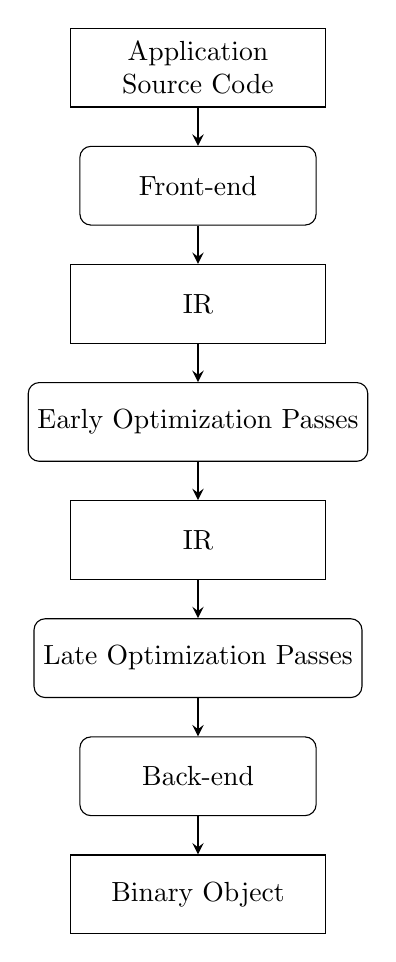
\begin{tikzpicture}[node distance=1.5cm]
            \node (start) [rect] {Application Source Code};
            \node (front-end) [rounded-rectangle, below of=start] {Front-end};
            \node (IR1) [rect, below of=front-end] {IR};
            \node (early-opt) [rounded-rectangle, below of=IR1] {Early Optimization Passes};
            \node (IR2) [rect, below of=early-opt] {IR};
            \node (late-opt) [rounded-rectangle, below of=IR2] {Late Optimization Passes};
            \node (back-end) [rounded-rectangle, below of=late-opt] {Back-end};
            \node (end) [rect, below of=back-end] {Binary Object};

            \draw [arrow] (start) -- (front-end);
            \draw [arrow] (front-end) -- (IR1);
            \draw [arrow] (IR1) -- (early-opt);
            \draw [arrow] (early-opt) -- (IR2);
            \draw [arrow] (IR2) -- (late-opt);
            \draw [arrow] (late-opt) -- (back-end);
            \draw [arrow] (back-end) -- (end);
        \end{tikzpicture}
    \end{figure}

    \newpage

    \bibliography{bibtex}{}
    \bibliographystyle{plain}

    \newpage

    \printindex
\end{document}